\documentclass{beamer}

\usetheme{Antibes}
\usepackage{verbatim}
\usecolortheme[RGB={120,0,0}]{structure}
\setbeamertemplate{blocks}[rounded][shadow=true]
\usepackage[utf8]{inputenc}

\usepackage{algorithm}
\usepackage[noend]{algpseudocode}

\beamertemplateballitem
% To number the references.
\setbeamertemplate{bibliography item}{\insertbiblabel}

\begin{document}

\title{UKP5: a New Algorithm for the Unbounded Knapsack Problem}
\author{Henrique Becker\footnote{From the Universidade Federal do Rio Grande do Sul\label{ft:ufrgs}} and Luciana S. Buriol\textsuperscript{\ref{ft:ufrgs}}\\
15th International Symposium on Experimental Algorithms\\
(SEA 2016)
}
\logo{
\includegraphics[scale=0.3]{inf}}
\date{Wednesday, June 8}

\frame{\titlepage}

\frame{\frametitle{Outline}\tableofcontents}

\section{Introduction}
\frame{\frametitle{What is UKP?}
\begin{itemize}
%\setlength\itemsep{1.5em}
%\item UKP is an acronym for Unbounded Knapsack Problem.
\item Very similar to BKP or 0-1 KP.
\begin{itemize}
\item But with an ``unbounded'' quantity of each item available.
\end{itemize}
\end{itemize}
\large
\begin{align}
  maximize &\sum_{i=1}^n p_i x_i\label{eq:objfun}\\
subject~to &\sum_{i=1}^n w_i x_i \leq c\label{eq:capcons}\\
            &x_i \in \mathbb{N}_0\label{eq:x_integer}
\end{align}
\normalsize
\begin{itemize}
\vspace{-7mm}
\item Subproblem of the column generation technique (often used to solve CSP/BPP).
\end{itemize}
}

%\frame{\frametitle{UKP Model}
%\LARGE
%\begin{align}
%  maximize &\sum_{i=1}^n p_i x_i\label{eq:objfun}\\
%subject~to &\sum_{i=1}^n w_i x_i \leq c\label{eq:capcons}\\
%            &x_i \in \mathbb{N}_0\label{eq:x_integer}
%\end{align}
%}

\section{Prior Work}
\frame{\frametitle{Methods on Solving UKP}
\begin{beamerboxesrounded}[shadow=true]{Dynamic Programming (DP)}
Strong correlation between variables \textbf{n} \& \textbf{c} and the time to solve.\\

\small
Ex.: Garfinkel\cite{gar72},  T.C. Hu\cite{tchu}, G\&G\cite{gg66}, Greenberg \& Feldman\cite{greenberg_improved_ukp5}, Greenberg\cite{greenberg_2}, EDUK\cite{eduk}.
\end{beamerboxesrounded}	
\vspace{2mm}
\begin{beamerboxesrounded}[shadow=true]{Branch and Bound (B\&B)}
Strong correlation between instance's distribution and time to solve.\\

\small
Ex.: G\&G\cite{gg63-bb}, MTU1\cite{mtu1}, MTU2\cite{mtu2}.
\end{beamerboxesrounded}	
}

\frame{\frametitle{EDUK2/PYAsUKP (State-of-art)}
\begin{beamerboxesrounded}[shadow=true]{Knapsack Problems, 2004}
``EDUK [...] seems to be the most efficient dynamic programming based method available at the moment.''\cite[p. 223]{knapsackproblems2004}
\end{beamerboxesrounded}
\begin{itemize}
\item EDUK2 is the algorithm, PYAsUKP is the only known implementation (OCaml). %(As the algorithm uses many functional concepts the authors found that it would be so much easier to implement the algorithm on a functional language. Even if c++ is the de facto language for scientific computing.)
\item \textbf{Hybrid Approach}: Tries to solve by B\&B, if fails to solve quickly then defaults to DP. %(Only hybrid method known.)
\end{itemize}
}

\section{UKP5}
\frame{\frametitle{UKP5}
\begin{itemize}
\item Simple DP algorithm based on the algorithm presented on \cite{gar72} (Garfinkel \& Nemhauser).
\begin{itemize}
  \item \textbf{Symmetry pruning} % symmetric solutions are pruned in a more efficient fashion than in~\cite{gar72};
  \item \textbf{Sparsity} % not every position of the optimal solutions value array has to be computed;
  \item \textbf{Dominated solutions pruning} % dominated solutions are pruned;
  \item \textbf{Time/memory tradeoff} % the test \(w_i \leq y\) from the algorithm in~~\cite{gar72} was removed in cost of more O(\(w_{max}\)) memory;
  \item \textbf{Periodicity} % the periodicity check suggested in~\cite{gar72} (but not implemented there) was adapted and implemented.
\end{itemize}
\end{itemize}
}

\frame{\frametitle{UKP5 Code}
%\scriptsize
\small
%\begin{algorithm}
%\caption{UKP5 -- Computation of $opt$}\label{alg:ukp5}
\begin{algorithmic}[1]
\Procedure{UKP5}{$n, c, w, p, w_{min}, w_{max}$}
  \State \(g \gets\) array of \(c + w_{max}\) positions each one initialized with \(0\)\label{create_g}
  \State \(d \gets\) array of \(c + w_{max}\) positions each one initialized with \(n\)\label{create_d}
  
  \For{\(i \gets 1, n\)}\label{begin_trivial_bounds}\Comment{Creates all single-item solutions}
    \If{\(g[w_i] < p_i\)}
      \State \(g[w_i] \gets p_i\)
      \State \(d[w_i] \gets i\)
    \EndIf
  \EndFor\label{end_trivial_bounds}

  \State \(opt \gets 0\)\label{init_opt}

  \For{\(y \gets w_{min}, c\)}\label{main_ext_loop_begin}\Comment{Iterate the stored solutions}
%    \If{\(g[y] \leq opt\)}\label{if_less_than_opt_begin}%\Comment{Handles sparsity and pruning of dominated solutions}
    	\State \textbf{if} \(g[y] \leq opt\) \textbf{then skips to next iteration}%\label{if_less_than_opt_begin}\label{alg:continue}%\Comment{Ends current iteration and begins the next}
%    \EndIf\label{if_less_than_opt_end}
    
    \State \(opt \gets g[y]\)\label{update_opt}
    
    \For{\(i=1,d[y]\)}\label{main_inner_loop_begin}\Comment{Combine current solution with items}
      \If{\(g[y + w_i] < g[y] + p_i\)}\label{if_new_lower_bound_begin}
        \State \(g[y + w_i] \gets g[y] + p_i\)
        \State \(d[y + w_i] \gets i\)
      \EndIf\label{if_new_lower_bound_end}
    \EndFor\label{main_inner_loop_end}
  \EndFor\label{main_ext_loop_end}
  \State \textbf{return} \(opt\)
\EndProcedure
\end{algorithmic}
%\end{algorithm}
}

\frame{\frametitle{GG66}
\begin{itemize}
\setlength\itemsep{1.5em}
\item ``Ordered Step-Off'': algorithm of Gilmore and Gomore (1966)\cite{gg66}.
\item Found after sending this paper to the symposium.%(We notified the conference chair, but the paper was already submited for printing.)
\item Basically the same algorithm than UKP5.%(only uses the own vector for storing the profit of the best solution, instead of one single variable)
\end{itemize}
}

\frame{\frametitle{GG66 Code}
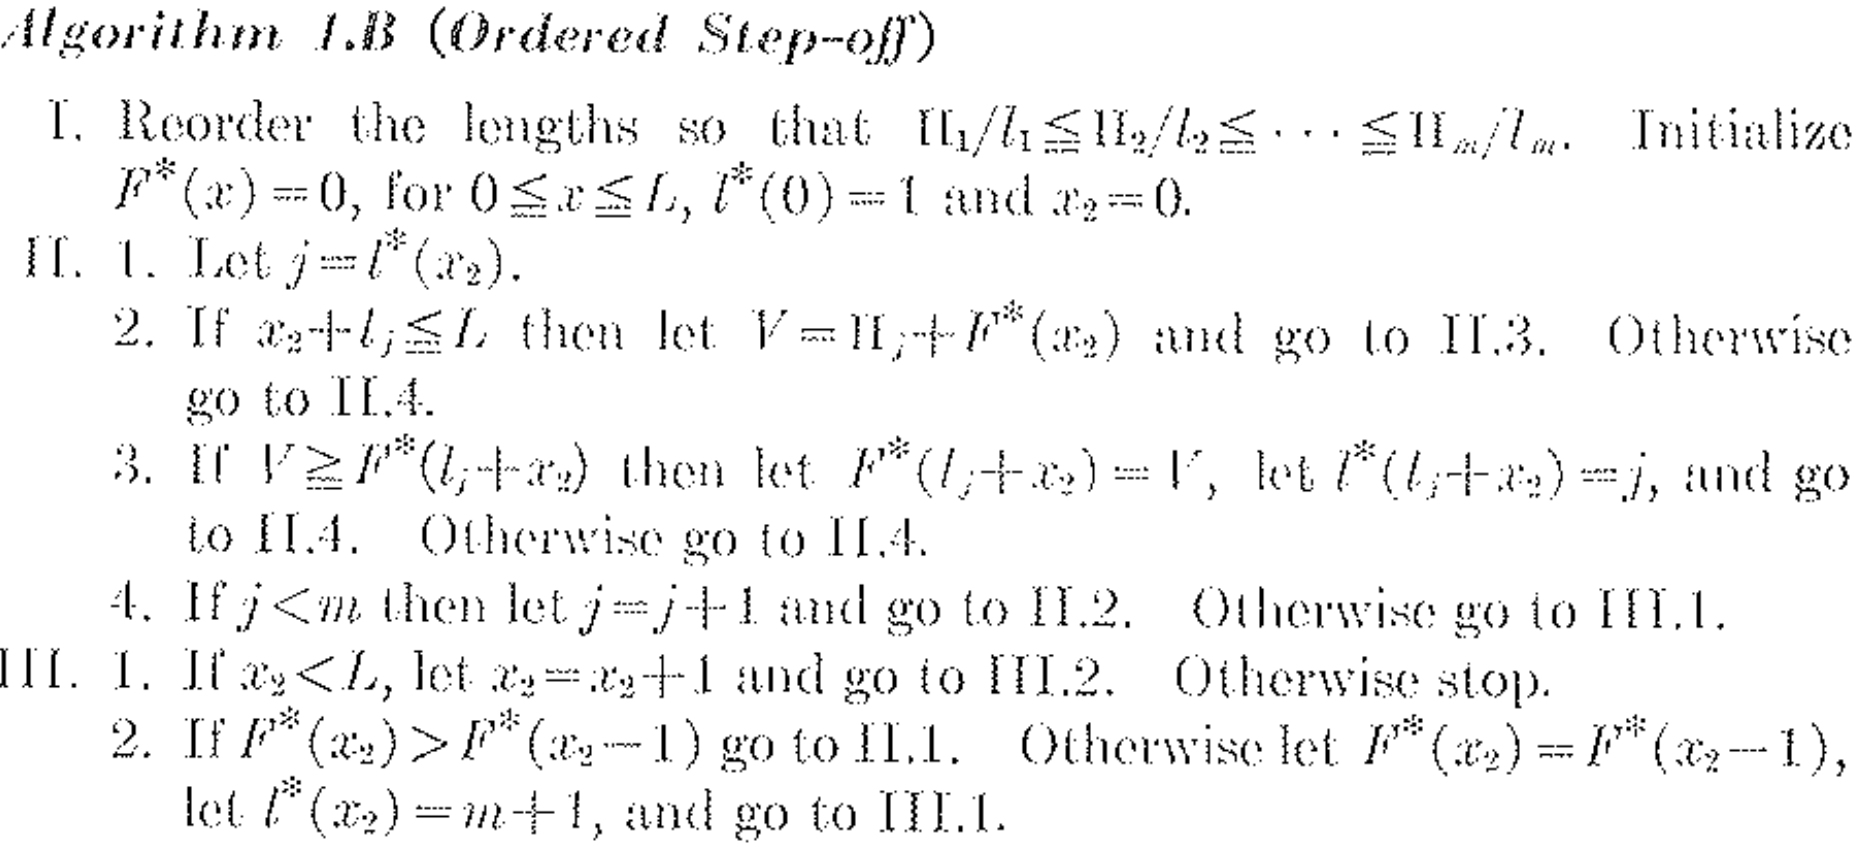
\includegraphics[scale=0.175]{gg66.png} 
}

\begin{comment}
\frame{\frametitle{GG66 Code 2}
Algorithm 1.B (Ordered Step-off)
\begin{itemize}
\item[I.] Reorder the lengths so that \(\pi_1/l_1 \leq \pi_2/l_2 \leq \dots \leq \pi_m/l_m\). Initialize \(F^*(x) = 0\), for \(0 \leq x \leq L\), \(l^*(0) = 1\) and \(x_2 = 0\).
\item[II.] \begin{itemize}
	\item[1] Let \(j = l^*(x_2)\).
	\item[2] If \(x_2 + l_j \leq L\) then let \(V = \pi_{j} + F^*(x_2)\) and go to II.3. Otherwise go to II.4.
	\item[3] If \(V \geq F^*(l_j+x_2)\) then let \(F^*(l_j+x_2) = V\), let \(l^*(l_j+x2) = j\), and go II.4. Otherwise go to II.4.
	\item[4] If \(j < m\) then let \(j = j + 1\) and go to II.2. Otherwise go to III.1.
\end{itemize}
\item[III.] \begin{itemize}
	\item[1] If \(x_2 < L\), let \(x_2 = x_2 + 1\) and go to III.2. Otherwise stop.
	\item[2] If \(F^*(x_2) > F^*(x_2 - 1)\) go to II.1. Otherwise let \(F^*(x_2) = F^*(x_2-1)\), let \(l^*(x_2) = m + 1\), and go to III.1.
\end{itemize}
\end{itemize}
}
\end{comment}

\frame{\frametitle{GG66 Code (changed notation)}
Algorithm 1.B (Ordered Step-off)
\begin{itemize}
\item[I.] Reorder the lenghts so that \(p_1/w_1 \leq p_2/w_2 \leq \dots \leq p_n/w_n\). Initialize \(F^*(y') = 0\), for \(0 \leq y' \leq c\), \(l^*(0) = 1\) and \(y = 0\).
\item[II.] \begin{itemize}
	\item[1] Let \(i = l^*(y)\).
	\item[2] If \(y + w_i \leq c\) then let \(v = p_i + F^*(y)\) and go to II.3. Otherwise go to II.4.
	\item[3] If \(v \geq F^*(y+w_i)\) then let \(F^*(y+w_i) = v\), let \(l^*(y+w_i) = i\), and go II.4. Otherwise go to II.4.
	\item[4] If \(i < n\) then let \(i = i + 1\) and go to II.2. Otherwise go to III.1.
\end{itemize}
\item[III.] \begin{itemize}
	\item[1] If \(y < c\), let \(y = y + 1\) and go to III.2. Otherwise stop.
	\item[2] If \(F^*(y) > F^*(y - 1)\) go to II.1. Otherwise let \(F^*(y) = F^*(y-1)\), let \(l^*(y) = n + 1\), and go to III.1.
\end{itemize}
\end{itemize}
}

\section{Experiments and Results}

\frame{\frametitle{The instances}
\begin{itemize}
\item A set of 4540 ``hard'' instances proposed in \cite{pya} (EDUK2 paper). %(Hard is a little complex to define here. Some formulae were proven to create instances that are hard to solve by B\&B (hard to reach upper bound); some are guaranteed to be resistent to methods that allow to reduce the number of items or the capacity of the instance).
\item Used the same tool and similar parameters to generate them. %(The tool is the own pyasukpt, that isn't only an implementation of the EDUK2 but also a implementation of many instance generators.)
\item Five different classes of instances.%(We adopted the same five classes used on PYAsUKP, and only augmented one of the classes because with the hardwere evolution it had become too easy to solve.)
\begin{itemize}
	\item Instances with no collective dominance;
	\item Instances with postponed periodicity;
	\item Strong correlated (profit and weight);
	\item SAW (proved to be hard to solved by B\&B\cite{chung});
	\item Subset~sum instances;
\end{itemize}
\end{itemize}
}

\begin{frame}
\frametitle{Times table}
\begin{tabular}{llllll}
%\multicolumn{2}{l}{} & \multicolumn{4}{l}{UKP5} & \multicolumn{4}{l}{PYAsUKP}\\
        &  & UKP5 & PYA & UKP5 & PYA\\ \hline
Class & Nº	& avg & avg & sd & sd \\ \hline
W.C.D. & 2000 	& \textbf{1.55} & 34.11 & \textbf{1.94} & 82.35 \\ \hline
S.S. & 400 	& \textbf{0.08} & 6.39 & \textbf{0.20} & 55.33 \\ \hline
S.C. & 240 	& \textbf{0.34} & 52.46 & \textbf{0.36} & 110.24 \\ \hline
SAW & 1100	& \textbf{3.10} & 15.43 & \textbf{5.35} & 31.82 \\ \hline
P.P. & 800 	& \textbf{5.01} & 121.71 & \textbf{3.81} & 173.30 \\
Class & Nº	& min & min & max & max \\ \hline
W.C.D. & 2000 	& 0.02 & \textbf{0.00} & \textbf{13.17} & 667.80 \\ \hline
S.S. & 400 	& 0.01 & \textbf{0.00} & \textbf{1.42} & 726.34 \\ \hline
S.C. & 240 	& 0.04 & \textbf{0.00} & \textbf{1.13} & 721.88 \\ \hline
SAW & 1100 	& 0.09 & \textbf{0.01} & \textbf{21.93} & 192.03 \\ \hline
P.P. & 800 	& 0.54 & \textbf{0.01} & \textbf{14.98} & 828.89 \\
%W.C.D. & 2000 & 1.5581567411 & 1.9448457081 & 0.0288475 & 13.1754 & 34.117780105 & 82.3560955348 & 0 & 667.80327 \\ \hline
%S.S. & 400 & 0.08 & 0.20 & 0.01 & 1.42 & 6.39 & 55.33 & 0.00 & 726.34 \\ \hline
%S.C. & 240 & 0.3468662025 & 0.3618682953 & 0.046731 & 1.13176 & 52.4671329583 & 110.2489829781 & 0 & 721.88659 \\ \hline
%SAW & 1100 & 3.1080885875 & 5.3562777737 & 0.0984506 & 21.9394 & 15.4338201 & 31.828562601 & 0.01333 & 192.03665 \\ \hline
%P.P. & 800 & 5.0175573 & 3.8174543896 & 0.549045 & 14.9801 & 121.7176255625 & 173.3084120879 & 0.01 & 828.89325 \\
\end{tabular}
% Create table? (Use many criteria? compute overall average; compute class average, then overal average; compute subclass averages, then overall average; compute subclass averages, then class aversages, then overall average)'
%Average of all instances: 18.5 % 18.5046187167
%Average of the classes averages (not-weighted): 55.65 % 55.6568069177
%Average of the subclasses average (not-weighted): 63.12 % 63.1277717668
%Weighted average of the classes averages (as subclasses averages): 46.88 %46.8856431027
\end{frame}

\frame{\frametitle{Times charts}
\centering
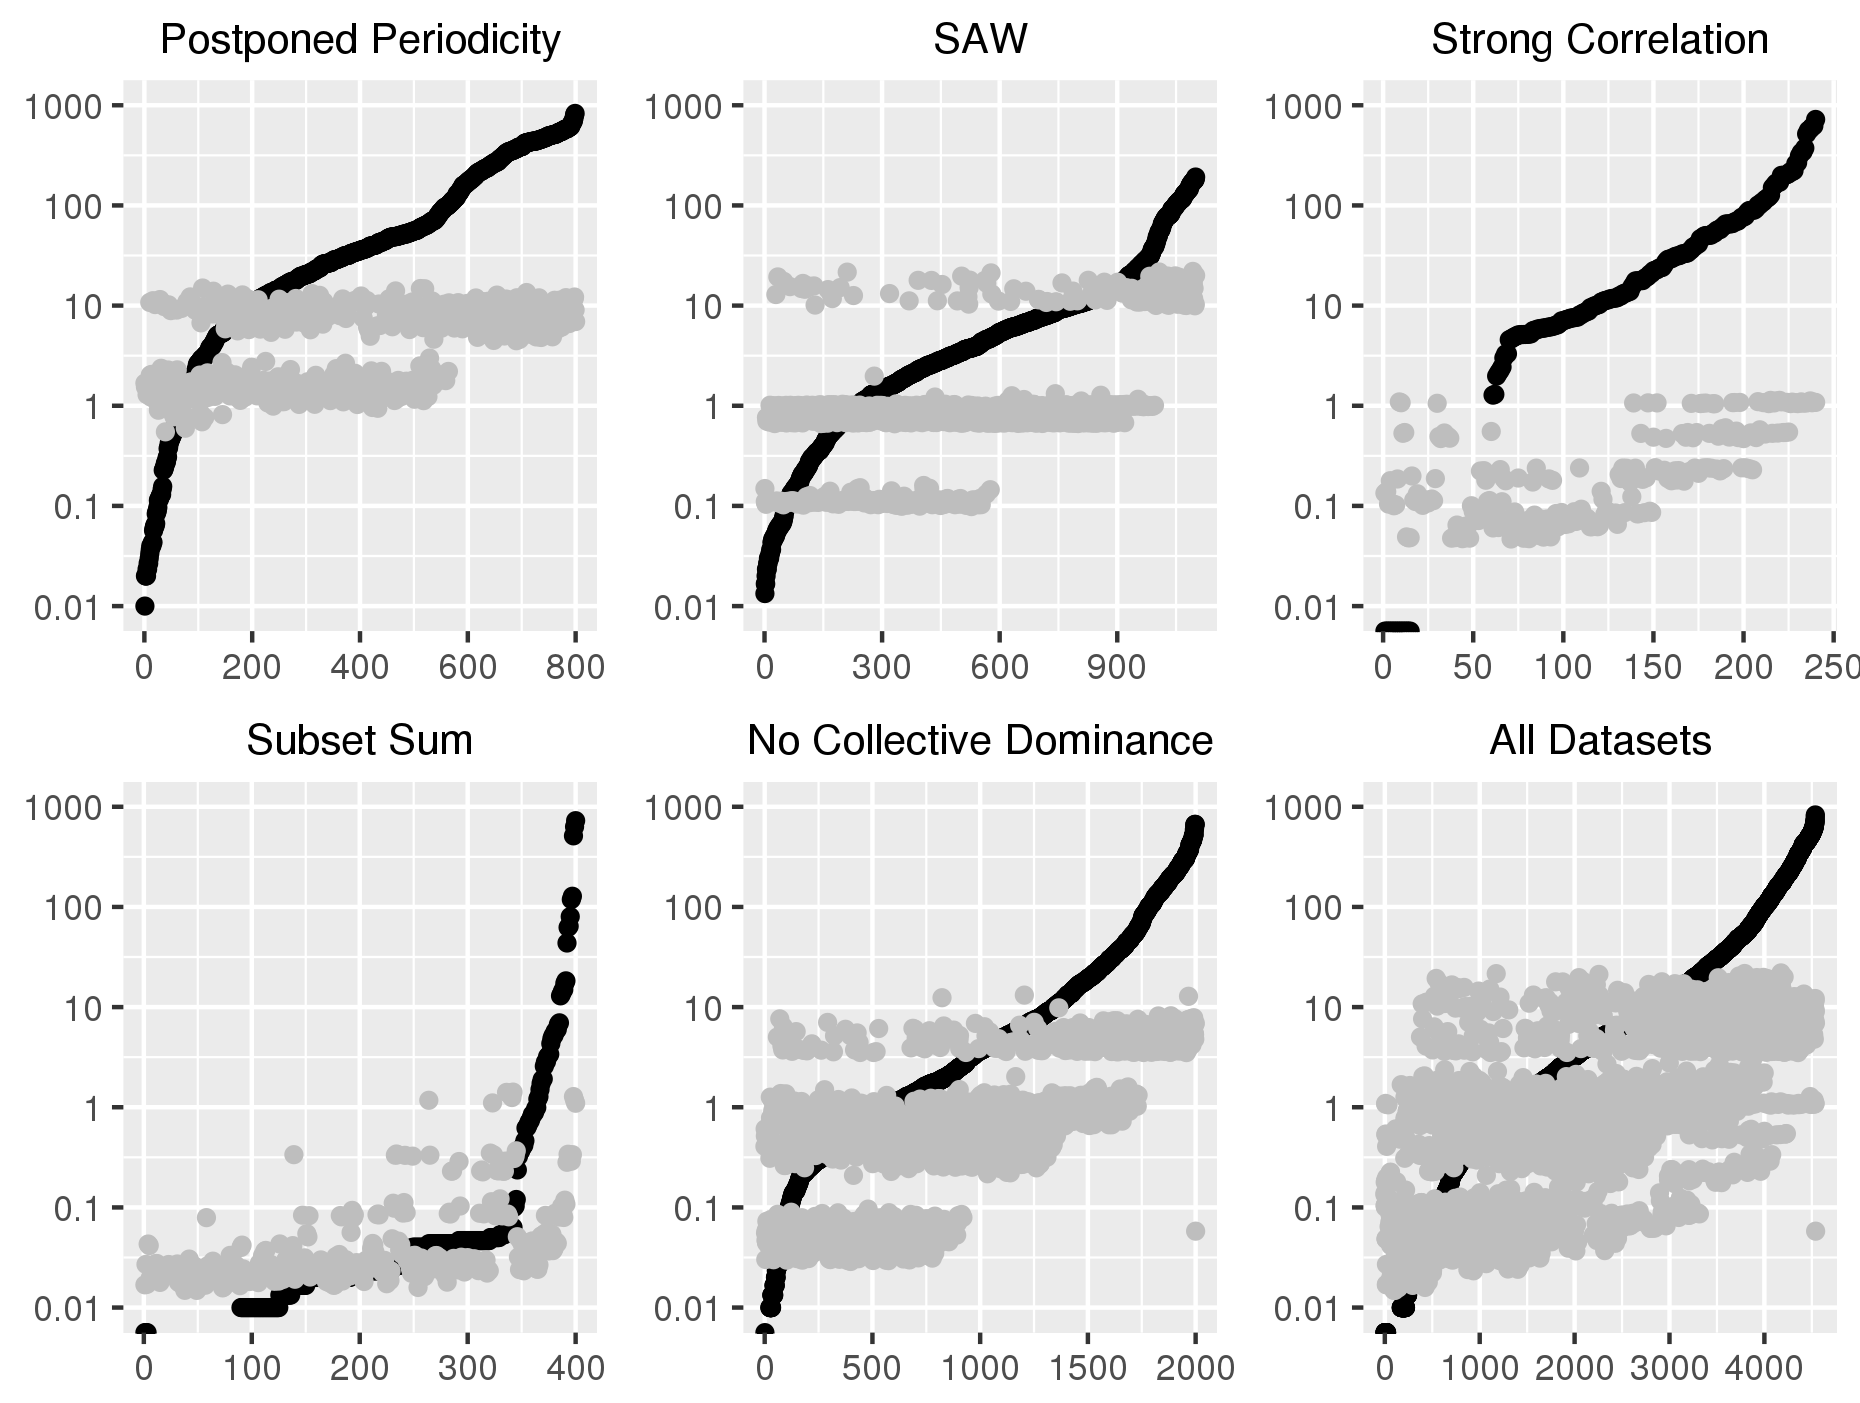
\includegraphics[scale=0.6]{six_plots.png} 
}

\frame{\frametitle{Times graph II}
\centering
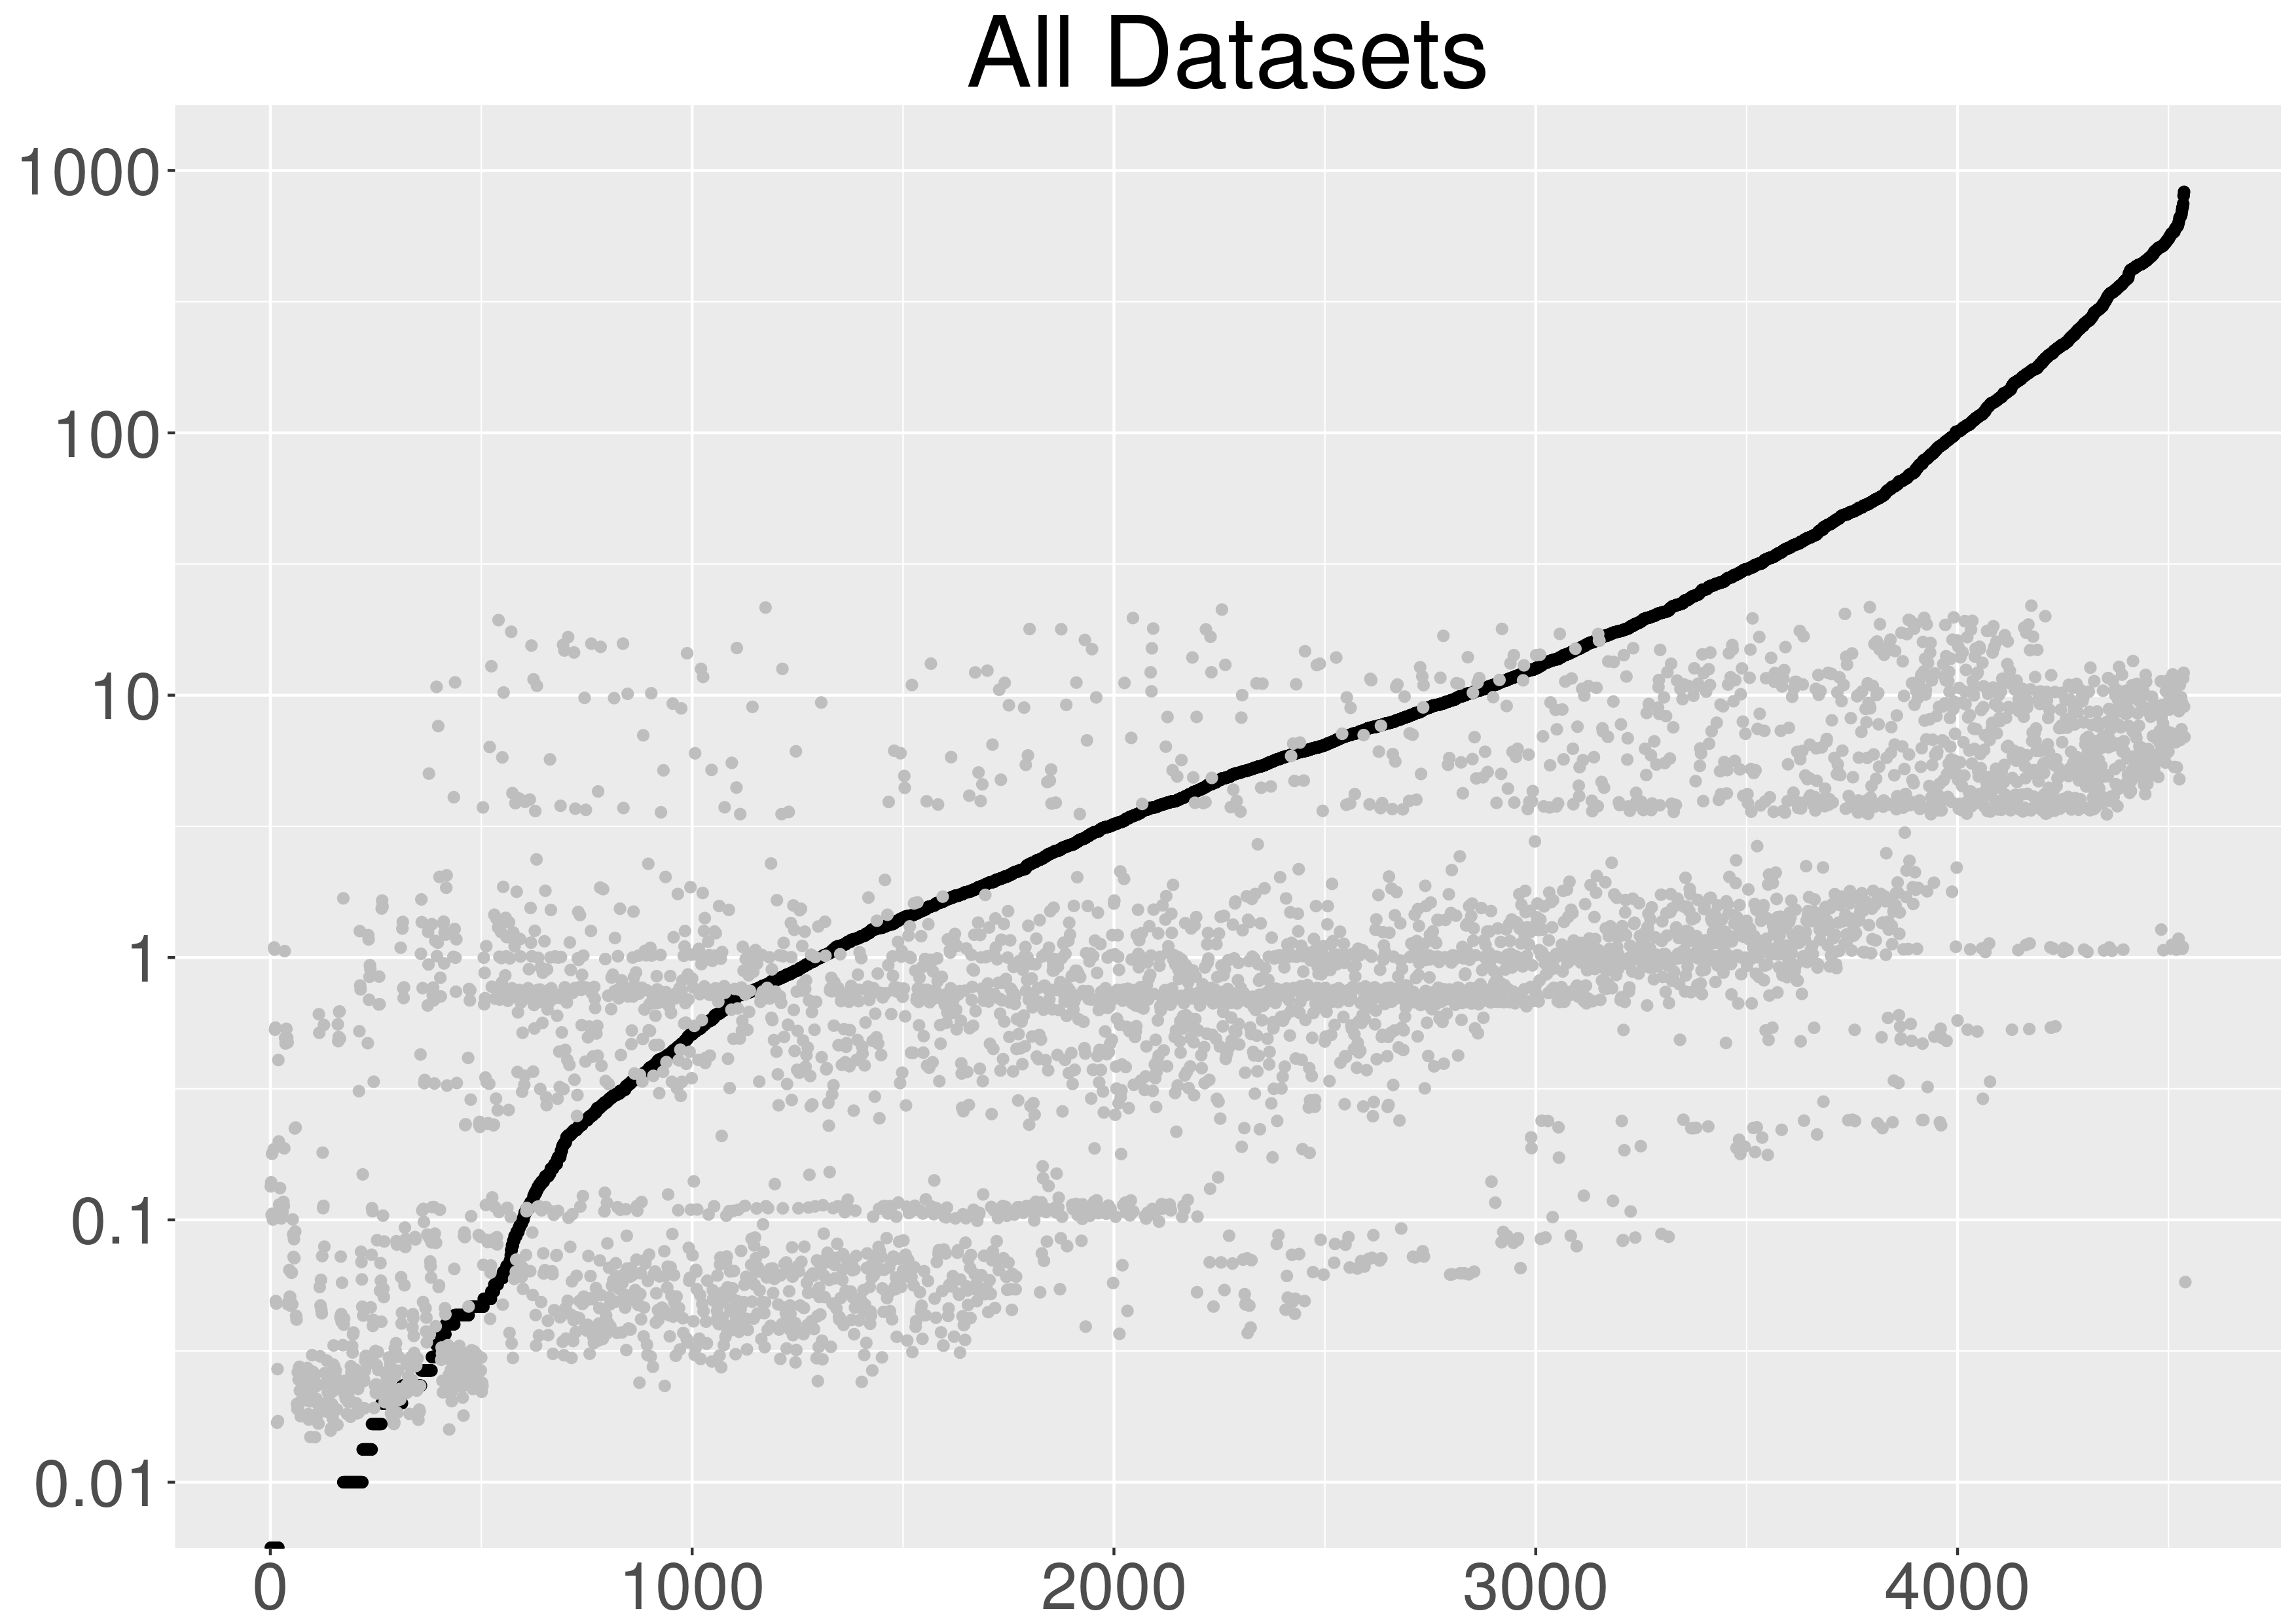
\includegraphics[scale=0.35]{all.png} 
}

\section{Analysis and Final Remarks}

\frame{\frametitle{Hard vs Easy -- DP vs B\&B}
\begin{itemize}
\setlength\itemsep{1.5em}
\item PYAsUKP is mainly a DP method. %(the cases where the B\&B don't solve the instance instantly, it don't affect the PYAsUKP time very much)
\item The benchmark proposed at PYAsUKP's paper focused hard-to-solve-by-B\&B instances. %(Instances with similar profit-to-weight ratio; them most efficient items being the ones with the biggest weight; etc..)
\item PYAsUKP results were compared against the ones from a B\&B method, and against no other DP method. % (the method was MTU2)
\end{itemize}
}

\frame{\frametitle{Final remarks}
\begin{itemize}
\setlength\itemsep{1.5em}
\item The algorithm isn't novel, but is ``faster'' than the ``state-of-art''. %(At least for the instances proposed by authors of the state-of-art themselves)
\item Except by PYAsUKP, DP algorithms were abandoned with almost no empiric evidence. %(No paper presenting a DP algorithm compared computational results with another DP algorithm. And no paper presenting a B\&B algorithm compared to DP (only to other B\&B).)
\item A clear definition of the usefulness of each approach is necessary. %(We need to know for what instance sizes and other instance characteristics each approach is better, and we need to base this on solid empiric evidence.)
\end{itemize}
}

\frame{\frametitle{Future Works}
\begin{beamerboxesrounded}[shadow=true]{A survey on the UKP}
\begin{itemize}
\item Improve the benchmark dataset. %(include very big and random instances; include instances generated by the CPS/BPP column generation; create instances so hard that will make UKP5 take more than 1000s)
\item Test old algorithms that were presented with no computational results. %(many were already implemented after we send the paper)
\item Point that UKP5/GG66 are the same algorithm.%, and apologize. %(avoid that the misconception created by our article become long-lived)
\end{itemize}
\end{beamerboxesrounded}	
}

\frame{\frametitle{Questions?}
\center
This is, if we have time yet.\\
%(Sorry for my terrible pronunciation.)
}

\bibliographystyle{splncs03.bst}

\begin{frame}[allowframebreaks]{References}
\bibliography{slides_sea2016.bib}
\end{frame}

\end{document}

